%----------------------------------------------------------------------------------------
%	PACKAGES AND DOCUMENT CONFIGURATIONS
%----------------------------------------------------------------------------------------
% !TEX root=main.tex
\documentclass[10pt,paper,trans]{IEEEtran}

\usepackage[utf8]{inputenc}
\usepackage{graphicx}
\usepackage[english,spanish,activeacute]{babel}
\usepackage[cmex10]{amsmath}
\usepackage{hyperref}
\hypersetup{
    colorlinks=true,
    linkcolor=blue,
    urlcolor=blue,
    citecolor=black
}

\usepackage[numbers]{natbib}
\usepackage{xurl}


\begin{document}

\newcommand{\titlepaper}{Least Squares Filter Applied to a Temperature Control System using Simulink}

\title{\titlepaper}

\selectlanguage{english}
\author{\IEEEauthorblockN{Erick Andrés Obregón Fonseca}

\IEEEauthorblockA{erickof@estudiantec.cr}
\IEEEauthorblockA{\\MSc in Electronics -- Microelectronics Emphasis}
\IEEEauthorblockA{\\Instituto Tecnológico de Costa Rica}
}


\markboth{Obregón-Fonseca, \titlepaper}
{Shell \MakeLowercase{\textit{et al.}}: Bare Demo of IEEEtran.cls for Journals}


\IEEEtitleabstractindextext{%

\renewcommand{\abstractname}{Abstract}

\begin{abstract}
Accurate temperature monitoring is crucial in numerous daily and industrial applications. To address this, the utilization of a least-squares filter to effectively mitigate noise in the measured variable is explored in this paper.

For the study, a heating system was simulated using Simulink, incorporating Gaussian white noise into the output to mirror real-world disturbances. The system maintains a set-point of 25$^\circ$C, which represents the ambient temperature, and features an input pulse that activates the heating mechanism.

The findings indicate that the least-squares estimation technique successfully approximates the actual temperature with a high degree of accuracy, achieving results that closely match the true values.
\end{abstract}


\renewcommand{\IEEEkeywordsname}{Keywords}

\begin{IEEEkeywords}
Control System, Least Squares Filter, Simulink, Temperature
\end{IEEEkeywords}}

\maketitle

\IEEEdisplaynontitleabstractindextext

\IEEEpeerreviewmaketitle

\selectlanguage{english}

\section{Introduction}
Heating and temperature control systems have played a crusial role since the end of the 19th century. This kind of system has different applications in day-to-day task and industrial applications.\\


In 1895, Johnson contributed to temperature control with an automatic multi-zone temperature control system~\cite{us542733s}.






\section{Methodology}


\section{Results and Discussion}



\begin{figure}[H]
    \centering
    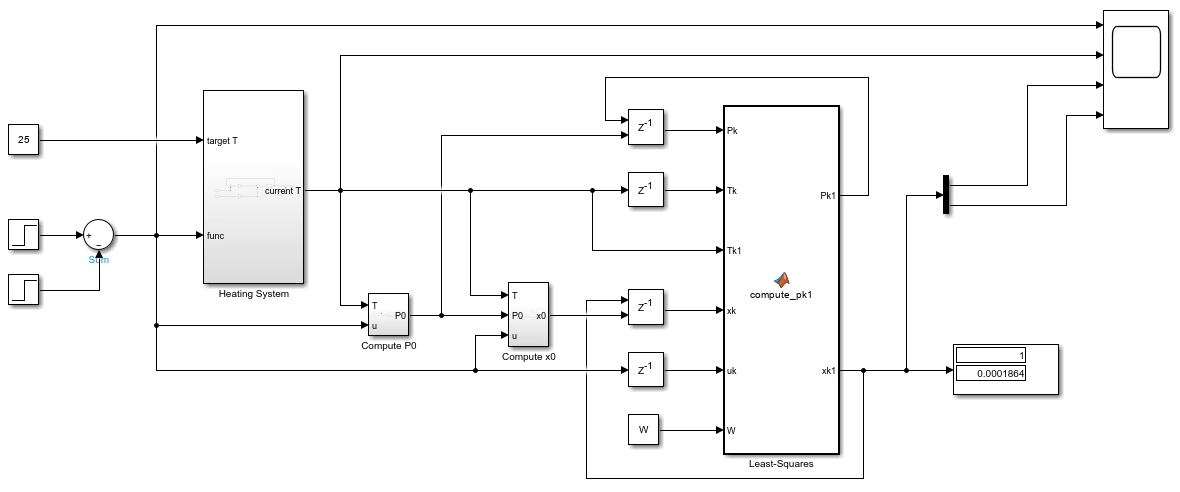
\includegraphics[width=1\linewidth]{figures/simulink_system.png}
    \caption{}
    \label{fig:simulink_system}
\end{figure}



\begin{figure}[H]
    \centering
    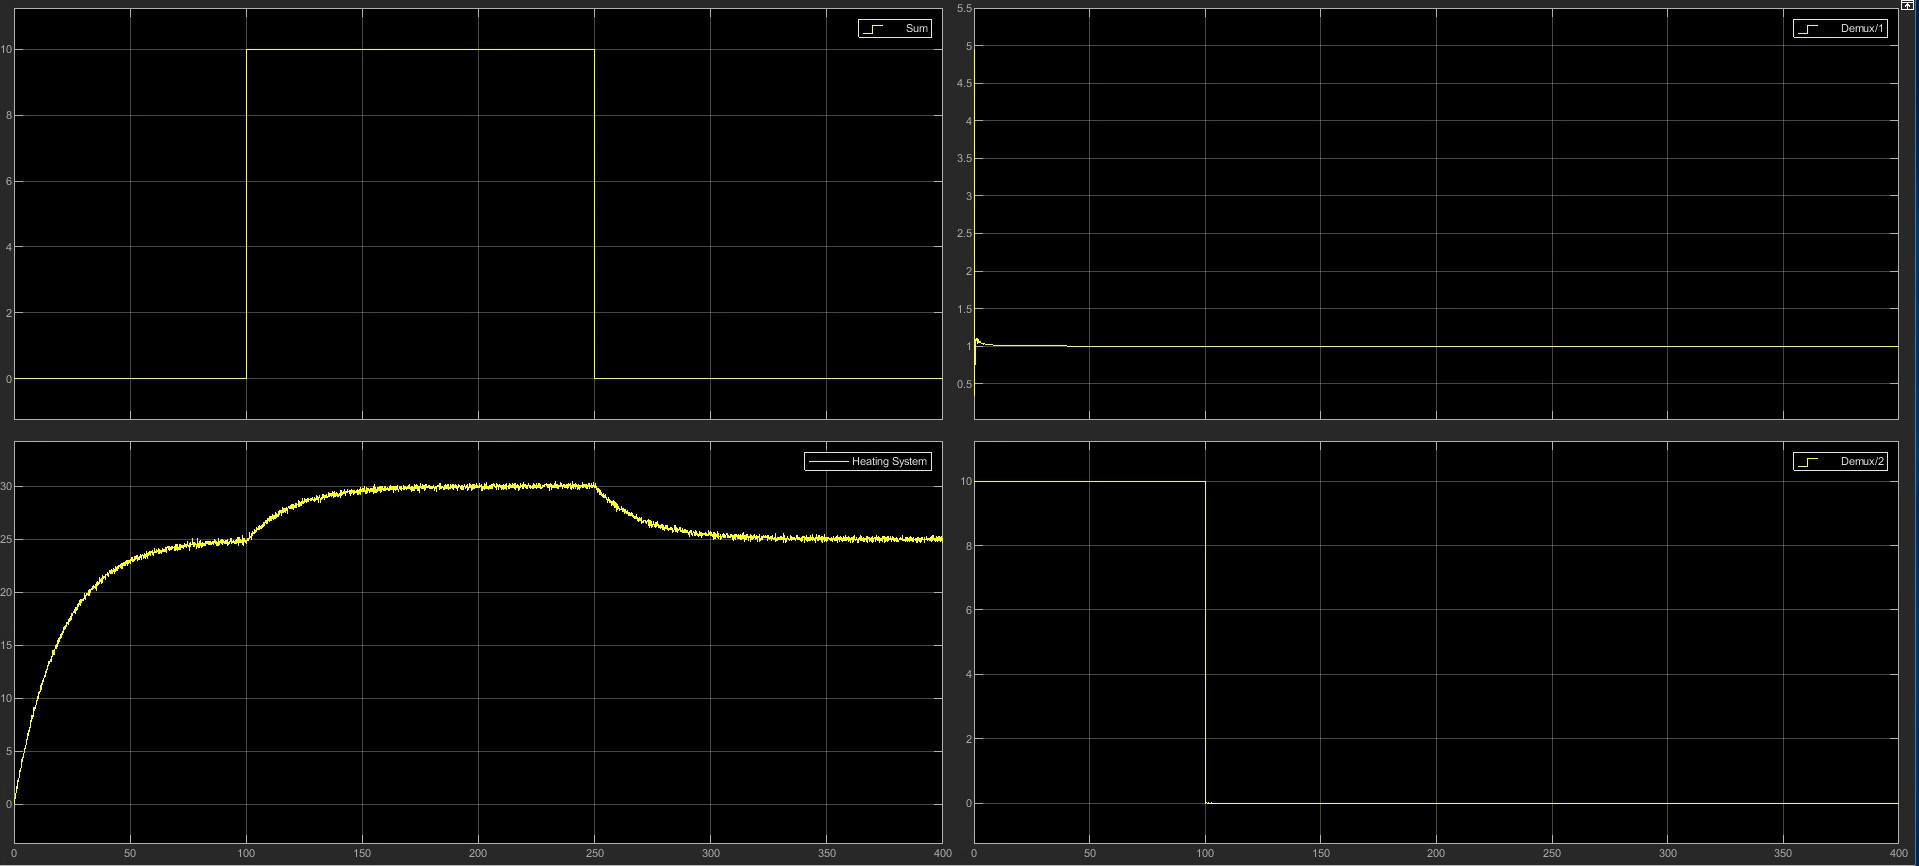
\includegraphics[width=1\linewidth]{figures/simulink_plot.png}
    \caption{}
    \label{fig:simulink_plot}
\end{figure}



\begin{figure}[H]
    \centering
    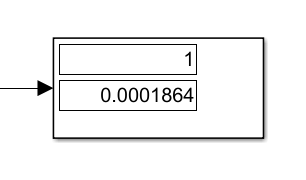
\includegraphics[width=0.7\linewidth]{figures/simulink_params.png}
    \caption{}
    \label{fig:simulink_params}
\end{figure}



\begin{figure}[H]
    \centering
    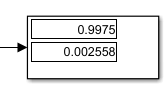
\includegraphics[width=0.5\linewidth]{figures/simulink_params_gen.png}
    \caption{}
    \label{fig:simulink_params_gen}
\end{figure}



\section{Conclusions}
Heating and temperature control systems play a crucial role in enhancing both energy efficiency and occupant comfort. Accurately controlling indoor temperatures is indispensable across several fields, including but not limited to biotechnology, biology, food supply chain, transportation, and automotive industries. These systems ensure optimal thermal comfort while providing a high degree of customization and flexibility to accommodate diverse user requirements and building characteristics. By minimizing energy wastage, they facilitate cost savings and contribute significantly to environmental sustainability efforts. \\

The least-squares filter exhibits remarkable robustness in handling data susceptible to random errors or fluctuations, showcasing its adaptability to diverse degrees of data complexity. While it excels in delivering accurate parameter estimations, particularly with large data, it does entail heightened computational demands as dataset size increases, necessitating careful resource allocation. Nevertheless, its versatility renders it invaluable across a wide range of fields and disciplines, underscoring its universal utility and relevance. \\

Simulink presents a robust platform for multi-domain modelling and simulation, empowering engineers and researchers to design and simulate complex systems that span multiple domains. Its intuitive graphical user interface and extensive library of pre-built blocks streamline the integration of diverse components and subsystems, facilitating accelerated prototyping and comprehensive system-level analysis and validation. With its user-friendly block diagram interface, users can quickly iterate on system designs, fine-tune parameters, and evaluate performance in real-time, thereby trimming development timelines and expenses. Furthermore, Simulink's seamless integration with MATLAB provides a cohesive environment for learning and applying computational techniques across various engineering and scientific disciplines.


\bibliographystyle{IEEEtranN}
\bibliography{bibliography/bibliography}

\end{document}
